\chapter{Functions}
\label{funcchap}

\section{Function calls}
\label{functionchap}
\index{function call}

In the context of programming, a {\bf function} is a named sequence of
statements that performs a computation.  When you define a function,
you specify the name and the sequence of statements.  Later, you can
``call'' the function by name.
We have already seen one example of a {\bf function call}:

\begin{verbatim}
>>> type(32)
<type 'int'>
\end{verbatim}
%
The name of the function is {\tt type}.  The expression in parentheses
is called the {\bf argument} of the function.  The result, for this
function, is the type of the argument.
\index{parentheses!argument in}

It is common to say that a function ``takes'' an argument and ``returns''
a result.  The result is called the {\bf return value}.
\index{argument}
\index{return value}


\section{Type conversion functions}
\index{conversion!type}
\index{type conversion}

% from Elkner:
% comment on whether these things are _really_ functions?
% use max as an example of a built-in?

% my reply:
% they are on the list of ``built-in functions'' so I am
% willing to call them functions.

Python provides built-in functions that convert values
from one type to another.  The {\tt int} function takes any value and
converts it to an integer, if it can, or complains otherwise:
\index{int function}
\index{function!int}

\begin{verbatim}
>>> int('32')
32
>>> int('Hello')
ValueError: invalid literal for int(): Hello
\end{verbatim}
%
{\tt int} can convert floating-point values to integers, but it
doesn't round off; it chops off the fraction part:

\begin{verbatim}
>>> int(3.99999)
3
>>> int(-2.3)
-2
\end{verbatim}
%
{\tt float} converts integers and strings to floating-point
numbers:
\index{float function}
\index{function!float}

\begin{verbatim}
>>> float(32)
32.0
>>> float('3.14159')
3.14159
\end{verbatim}
%
Finally, {\tt str} converts its argument to a string:
\index{str function}
\index{function!str}

\begin{verbatim}
>>> str(32)
'32'
>>> str(3.14159)
'3.14159'
\end{verbatim}
%



\section{Math functions}
\index{math function}
\index{function, math}

Python has a math module that provides most of the familiar
mathematical functions.  A {\bf module} is a file that contains a
collection of related functions.
\index{module}
\index{module object}

Before we can use the module, we have to import it:

\begin{verbatim}
>>> import math
\end{verbatim}
%
This statement creates a {\bf module object} named math.  If
you print the module object, you get some information about it:

\begin{verbatim}
>>> print math
<module 'math' (built-in)>
\end{verbatim}
%
The module object contains the functions and variables defined in the
module.  To access one of the functions, you have to specify the name
of the module and the name of the function, separated by a dot (also
known as a period).  This format is called {\bf dot notation}.
\index{dot notation}

\begin{verbatim}
>>> ratio = signal_power / noise_power
>>> decibels = 10 * math.log10(ratio)

>>> radians = 0.7
>>> height = math.sin(radians)
\end{verbatim}
%
The first example uses \verb"log10" to compute
a signal-to-noise ratio in decibels (assuming that \verb"signal_power" and
\verb"noise_power" are defined).  The math module also provides {\tt log},
which computes logarithms base {\tt e}.
\index{log function}
\index{function!log}
\index{sine function}
\index{radian}
\index{trigonometric function}
\index{function, trigonometric}

The second example finds the sine of {\tt radians}.  The name of the
variable is a hint that {\tt sin} and the other trigonometric
functions ({\tt cos}, {\tt tan}, etc.)  take arguments in radians. To
convert from degrees to radians, divide by 360 and multiply by
$2 \pi$:

\begin{verbatim}
>>> degrees = 45
>>> radians = degrees / 360.0 * 2 * math.pi
>>> math.sin(radians)
0.707106781187
\end{verbatim}
%
The expression {\tt math.pi} gets the variable {\tt pi} from the math
module.  The value of this variable is an approximation
of $\pi$, accurate to about 15 digits.
\index{pi}

If you know
your trigonometry, you can check the previous result by comparing it to
the square root of two divided by two:
\index{sqrt function}
\index{function!sqrt}

\begin{verbatim}
>>> math.sqrt(2) / 2.0
0.707106781187
\end{verbatim}
%

\section{Composition}
\index{composition}

So far, we have looked at the elements of a program---variables,
expressions, and statements---in isolation, without talking about how to
combine them.

One of the most useful features of programming languages is their
ability to take small building blocks and {\bf compose} them.  For
example, the argument of a function can be any kind of expression,
including arithmetic operators:

\begin{verbatim}
x = math.sin(degrees / 360.0 * 2 * math.pi)
\end{verbatim}
%
And even function calls:

\begin{verbatim}
x = math.exp(math.log(x+1))
\end{verbatim}
%
Almost anywhere you can put a value, you can put an arbitrary
expression, with one exception: the left side of an assignment
statement has to be a variable name.  Any other expression on the left
side is a syntax error (we will see exceptions to this rule
later).

\begin{verbatim}
>>> minutes = hours * 60                 # right
>>> hours * 60 = minutes                 # wrong!
SyntaxError: can't assign to operator
\end{verbatim}
%
\index{SyntaxError}
\index{exception!SyntaxError}


\section{Adding new functions}

So far, we have only been using the functions that come with Python,
but it is also possible to add new functions.
A {\bf function definition} specifies the name of a new function and
the sequence of statements that execute when the function is called.
\index{function}
\index{function definition}
\index{definition!function}

Here is an example:

\begin{verbatim}
def print_lyrics():
    print "I'm a lumberjack, and I'm okay."
    print "I sleep all night and I work all day."
\end{verbatim}
%
{\tt def} is a keyword that indicates that this is a function
definition.  The name of the function is \verb"print_lyrics".  The
rules for function names are the same as for variable names: letters,
numbers and some punctuation marks are legal, but the first character
can't be a number.  You can't use a keyword as the name of a function,
and you should avoid having a variable and a function with the same
name.
\index{def keyword}
\index{keyword!def}
\index{argument}

The empty parentheses after the name indicate that this function
doesn't take any arguments.
\index{parentheses!empty}
\index{header}
\index{body}
\index{indentation}
\index{colon}

The first line of the function definition is called the {\bf header};
the rest is called the {\bf body}.  The header has to end with a colon
and the body has to be indented.  By convention, the indentation is
always four spaces (see Section~\ref{editor}).  The body can contain
any number of statements.

The strings in the print statements are enclosed in double
quotes.  Single quotes and double quotes do the same thing;
most people use single quotes except in cases like this where
a single quote (which is also an apostrophe) appears in the string.
\index{ellipses}

If you type a function definition in interactive mode, the interpreter
prints ellipses ({\em ...}) to let you know that the definition
isn't complete:

\begin{verbatim}
>>> def print_lyrics():
...     print "I'm a lumberjack, and I'm okay."
...     print "I sleep all night and I work all day."
...
\end{verbatim}
%
To end the function, you have to enter an empty line (this is
not necessary in a script).

Defining a function creates a variable with the same name.

\begin{verbatim}
>>> print print_lyrics
<function print_lyrics at 0xb7e99e9c>
>>> type(print_lyrics)
<type 'function'>
\end{verbatim}
%
The value of \verb"print_lyrics" is a {\bf function object}, which
has type \verb"'function'".
\index{function object}
\index{object!function}

The syntax for calling the new function is the same as
for built-in functions:

\begin{verbatim}
>>> print_lyrics()
I'm a lumberjack, and I'm okay.
I sleep all night and I work all day.
\end{verbatim}
%
Once you have defined a function, you can use it inside another
function.  For example, to repeat the previous refrain, we could write
a function called \verb"repeat_lyrics":

\begin{verbatim}
def repeat_lyrics():
    print_lyrics()
    print_lyrics()
\end{verbatim}
%
And then call \verb"repeat_lyrics":

\begin{verbatim}
>>> repeat_lyrics()
I'm a lumberjack, and I'm okay.
I sleep all night and I work all day.
I'm a lumberjack, and I'm okay.
I sleep all night and I work all day.
\end{verbatim}
%
But that's not really how the song goes.


\section{Definitions and uses}
\index{function definition}

Pulling together the code fragments from the previous section, the
whole program looks like this:

\begin{verbatim}
def print_lyrics():
    print "I'm a lumberjack, and I'm okay."
    print "I sleep all night and I work all day."

def repeat_lyrics():
    print_lyrics()
    print_lyrics()

repeat_lyrics()
\end{verbatim}
%
This program contains two function definitions: \verb"print_lyrics" and
\verb"repeat_lyrics".  Function definitions get executed just like other
statements, but the effect is to create function objects.  The statements
inside the function do not get executed until the function is called, and
the function definition generates no output.
\index{use before def}

As you might expect, you have to create a function before you can
execute it.  In other words, the function definition has to be
executed before the first time it is called.

\begin{exercise}

Move the last line of this program
to the top, so the function call appears before the definitions. Run
the program and see what error
message you get.

\end{exercise}

\begin{exercise}

Move the function call back to the bottom
and move the definition of \verb"print_lyrics" after the definition of
\verb"repeat_lyrics".  What happens when you run this program?

\end{exercise}


\section{Flow of execution}
\index{flow of execution}

In order to ensure that a function is defined before its first use,
you have to know the order in which statements are executed, which is
called the {\bf flow of execution}.

Execution always begins at the first statement of the program.
Statements are executed one at a time, in order from top to bottom.

Function definitions do not alter the flow of execution of the
program, but remember that statements inside the function are not
executed until the function is called.

A function call is like a detour in the flow of execution. Instead of
going to the next statement, the flow jumps to the body of
the function, executes all the statements there, and then comes back
to pick up where it left off.

That sounds simple enough, until you remember that one function can
call another.  While in the middle of one function, the program might
have to execute the statements in another function. But while
executing that new function, the program might have to execute yet
another function!

Fortunately, Python is good at keeping track of where it is, so each
time a function completes, the program picks up where it left off in
the function that called it.  When it gets to the end of the program,
it terminates.

What's the moral of this sordid tale?  When you read a program, you
don't always want to read from top to bottom.  Sometimes it makes
more sense if you follow the flow of execution.


\section{Parameters and arguments}
\label{parameters}
\index{parameter}
\index{function parameter}
\index{argument}
\index{function argument}

Some of the built-in functions we have seen require arguments.  For
example, when you call {\tt math.sin} you pass a number
as an argument.  Some functions take more than one argument:
{\tt math.pow} takes two, the base and the exponent.

Inside the function, the arguments are assigned to
variables called {\bf parameters}.  Here is an example of a
user-defined function that takes an argument:
\index{parentheses!parameters in}

\begin{verbatim}
def print_twice(bruce):
    print bruce
    print bruce
\end{verbatim}
%
This function assigns the argument to a parameter
named {\tt bruce}.  When the function is called, it prints the value of
the parameter (whatever it is) twice.

This function works with any value that can be printed.

\begin{verbatim}
>>> print_twice('Spam')
Spam
Spam
>>> print_twice(17)
17
17
>>> print_twice(math.pi)
3.14159265359
3.14159265359
\end{verbatim}
%
The same rules of composition that apply to built-in functions also
apply to user-defined functions, so we can use any kind of expression
as an argument for \verb"print_twice":
\index{composition}

\begin{verbatim}
>>> print_twice('Spam '*4)
Spam Spam Spam Spam
Spam Spam Spam Spam
>>> print_twice(math.cos(math.pi))
-1.0
-1.0
\end{verbatim}
%
The argument is evaluated before the function is called, so
in the examples the expressions \verb"'Spam '*4" and
{\tt math.cos(math.pi)} are only evaluated once.
\index{argument}

You can also use a variable as an argument:

\begin{verbatim}
>>> michael = 'Eric, the half a bee.'
>>> print_twice(michael)
Eric, the half a bee.
Eric, the half a bee.
\end{verbatim}
%
The name of the variable we pass as an argument ({\tt michael}) has
nothing to do with the name of the parameter ({\tt bruce}).  It
doesn't matter what the value was called back home (in the caller);
here in \verb"print_twice", we call everybody {\tt bruce}.


\section{Variables and parameters are local}
\index{local variable}
\index{variable!local}

When you create a variable inside a function, it is {\bf local},
which means that it only
exists inside the function.  For example:
\index{parentheses!parameters in}

\begin{verbatim}
def cat_twice(part1, part2):
    cat = part1 + part2
    print_twice(cat)
\end{verbatim}
%
This function takes two arguments, concatenates them, and prints
the result twice.  Here is an example that uses it:
\index{concatenation}

\begin{verbatim}
>>> line1 = 'Bing tiddle '
>>> line2 = 'tiddle bang.'
>>> cat_twice(line1, line2)
Bing tiddle tiddle bang.
Bing tiddle tiddle bang.
\end{verbatim}
%
When \verb"cat_twice" terminates, the variable {\tt cat}
is destroyed.  If we try to print it, we get an exception:
\index{NameError}
\index{exception!NameError}

\begin{verbatim}
>>> print cat
NameError: name 'cat' is not defined
\end{verbatim}
%
Parameters are also local.
For example, outside \verb"print_twice", there is no
such thing as {\tt bruce}.
\index{parameter}


\section{Stack diagrams}
\label{stackdiagram}
\index{stack diagram}
\index{function frame}
\index{frame}

To keep track of which variables can be used where, it is sometimes
useful to draw a {\bf stack diagram}.  Like state diagrams, stack
diagrams show the value of each variable, but they also show the
function each variable belongs to.
\index{stack diagram}
\index{diagram!stack}

Each function is represented by a {\bf frame}.  A frame is a box
with the name of a function
beside it and the parameters and variables of the function inside it.
The stack diagram for the
previous example is shown in Figure~\ref{fig.stack}.

\begin{figure}
\centerline
{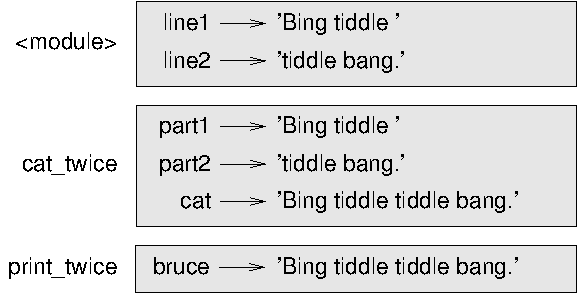
\includegraphics[scale=0.8]{figs/stack.pdf}}
\caption{Stack diagram.}
\label{fig.stack}
\end{figure}


The frames are arranged in a stack that indicates which function
called which, and so on.  In this example, \verb"print_twice"
was called by \verb"cat_twice", and \verb"cat_twice" was called by
\verb"__main__", which is a special name for the topmost frame.  When
you create a variable outside of any function, it belongs to
\verb"__main__".

Each parameter refers to the same value as its corresponding
argument.  So, {\tt part1} has the same value as
{\tt line1}, {\tt part2} has the same value as {\tt line2},
and {\tt bruce} has the same value as {\tt cat}.

If an error occurs during a function call, Python prints the
name of the function, and the name of the function that called
it, and the name of the function that called {\em that}, all the
way back to \verb"__main__".

For example, if you try to access {\tt cat} from within
\verb"print_twice", you get a {\tt NameError}:

\begin{verbatim}
Traceback (innermost last):
  File "test.py", line 13, in __main__
    cat_twice(line1, line2)
  File "test.py", line 5, in cat_twice
    print_twice(cat)
  File "test.py", line 9, in print_twice
    print cat
NameError: name 'cat' is not defined
\end{verbatim}
%
This list of functions is called a {\bf traceback}.  It tells you what
program file the error occurred in, and what line, and what functions
were executing at the time.  It also shows the line of code that
caused the error.
\index{traceback}

The order of the functions in the traceback is the same as the
order of the frames in the stack diagram.  The function that is
currently running is at the bottom.


\section{Fruitful functions and void functions}
\index{fruitful function}
\index{void function}
\index{function, fruitful}
\index{function, void}

Some of the functions we are using, such as the math functions, yield
results; for lack of a better name, I call them {\bf fruitful
  functions}.  Other functions, like \verb"print_twice", perform an
action but don't return a value.  They are called {\bf void
  functions}.

When you call a fruitful function, you almost always
want to do something with the result; for example, you might
assign it to a variable or use it as part of an expression:

\begin{verbatim}
x = math.cos(radians)
golden = (math.sqrt(5) + 1) / 2
\end{verbatim}
%
When you call a function in interactive mode, Python displays
the result:

\begin{verbatim}
>>> math.sqrt(5)
2.2360679774997898
\end{verbatim}
%
But in a script, if you call a fruitful function all by itself,
the return value is lost forever!

\begin{verbatim}
math.sqrt(5)
\end{verbatim}
%
This script computes the square root of 5, but since it doesn't store
or display the result, it is not very useful.
\index{interactive mode}
\index{script mode}

Void functions might display something on the screen or have some
other effect, but they don't have a return value.  If you try to
assign the result to a variable, you get a special value called
{\tt None}.
\index{None special value}
\index{special value!None}

\begin{verbatim}
>>> result = print_twice('Bing')
Bing
Bing
>>> print result
None
\end{verbatim}
%
The value {\tt None} is not the same as the string \verb"'None'".
It is a special value that has its own type:

\begin{verbatim}
>>> print type(None)
<type 'NoneType'>
\end{verbatim}
%
The functions we have written so far are all void.  We will start
writing fruitful functions in a few chapters.


\section{Why functions?}
\index{function, reasons for}

It may not be clear why it is worth the trouble to divide
a program into functions.  There are several reasons:

\begin{itemize}

\item Creating a new function gives you an opportunity to name a group
of statements, which makes your program easier to read and debug.

\item Functions can make a program smaller by eliminating repetitive
code.  Later, if you make a change, you only have
to make it in one place.

\item Dividing a long program into functions allows you to debug the
parts one at a time and then assemble them into a working whole.

\item Well-designed functions are often useful for many programs.
Once you write and debug one, you can reuse it.

\end{itemize}


\section{Importing with {\tt from}}

Python provides two ways to import modules; we have already seen one:

\begin{verbatim}
>>> import math
>>> print math
<module 'math' (built-in)>
>>> print math.pi
3.14159265359
\end{verbatim}
%
If you import {\tt math}, you get a module object named {\tt math}.
The module object contains constants like {\tt pi} and functions
like {\tt sin} and {\tt exp}.

But if you try to access {\tt pi} directly, you get an error.

\begin{verbatim}
>>> print pi
Traceback (most recent call last):
  File "<stdin>", line 1, in <module>
NameError: name 'pi' is not defined
\end{verbatim}
%
As an alternative, you can import an object from a module like this:

\begin{verbatim}
>>> from math import pi
\end{verbatim}
%
Now you can access {\tt pi} directly, without dot notation.
\index{dot notation}

\begin{verbatim}
>>> print pi
3.14159265359
\end{verbatim}
%
Or you can use the star operator to import {\it everything} from the
module:

\begin{verbatim}
>>> from math import *
>>> cos(pi)
-1.0
\end{verbatim}

The advantage of importing everything from the math module is that your
code can be more concise.  The disadvantage is that there might be
conflicts between names defined in different modules, or between
a name from a module and one of your variables.


\section{Debugging}
\label{editor}
\index{debugging}

If you are using a text editor to write your scripts, you might
run into problems with spaces and tabs.  The best way to avoid
these problems is to use spaces exclusively (no tabs).  Most text
editors that know about Python do this by default, but some
don't.
\index{whitespace}

Tabs and spaces are usually invisible, which makes them
hard to debug, so try to find an editor that manages indentation
for you.

Also, don't forget to save your program before you run it.  Some
development environments do this automatically, but some don't.
In that case the program you are looking at in the text editor
is not the same as the program you are running.

Debugging can take a long time if you keep running the same,
incorrect, program over and over!

Make sure that the code you are looking at is the code you are running.
If you're not sure, put something like \verb"print 'hello'" at the
beginning of the program and run it again.  If you don't see
\verb"hello", you're not running the right program!




\section{Glossary}

\begin{description}

\item[function:] A named sequence of statements that performs some
useful operation.  Functions may or may not take arguments and may or
may not produce a result.
\index{function}

\item[function definition:]  A statement that creates a new function,
specifying its name, parameters, and the statements it executes.
\index{function definition}

\item[function object:]  A value created by a function definition.
The name of the function is a variable that refers to a function
object.
\index{function definition}

\item[header:] The first line of a function definition.
\index{header}

\item[body:] The sequence of statements inside a function definition.
\index{body}

\item[parameter:] A name used inside a function to refer to the value
passed as an argument.
\index{parameter}

\item[function call:] A statement that executes a function. It
consists of the function name followed by an argument list.
\index{function call}

\item[argument:]  A value provided to a function when the function is called.
This value is assigned to the corresponding parameter in the function.
\index{argument}

\item[local variable:]  A variable defined inside a function.  A local
variable can only be used inside its function.
\index{local variable}

\item[return value:]  The result of a function.  If a function call
is used as an expression, the return value is the value of
the expression.
\index{return value}

\item[fruitful function:] A function that returns a value.
\index{fruitful function}

\item[void function:] A function that doesn't return a value.
\index{void function}

\item[module:] A file that contains a
collection of related functions and other definitions.
\index{module}

\item[import statement:] A statement that reads a module file and creates
a module object.
\index{import statement}
\index{statement!import}

\item[module object:] A value created by an {\tt import} statement
that provides access to the values defined in a module.
\index{module}

\item[dot notation:]  The syntax for calling a function in another
module by specifying the module name followed by a dot (period) and
the function name.
\index{dot notation}

\item[composition:] Using an expression as part of a larger expression,
or a statement as part of a larger statement.
\index{composition}

\item[flow of execution:]  The order in which statements are executed during
a program run.
\index{flow of execution}

\item[stack diagram:]  A graphical representation of a stack of functions,
their variables, and the values they refer to.
\index{stack diagram}

\item[frame:]  A box in a stack diagram that represents a function call.
It contains the local variables and parameters of the function.
\index{function frame}
\index{frame}

\item[traceback:]  A list of the functions that are executing,
printed when an exception occurs.
\index{traceback}


\end{description}


\section{Exercises}

\begin{exercise}
\index{len function}
\index{function!len}

Python provides a built-in function called {\tt len} that
returns the length of a string, so the value of \verb"len('allen')" is 5.

Write a function named \verb"right_justify" that takes a string
named {\tt s} as a parameter and prints the string with enough
leading spaces so that the last letter of the string is in column 70
of the display.

\begin{verbatim}
>>> right_justify('allen')
                                                                 allen
\end{verbatim}

\end{exercise}


\begin{exercise}
\index{function object}
\index{object!function}

A function object is a value you can assign to a variable
or pass as an argument.  For example, \verb"do_twice" is a function
that takes a function object as an argument and calls it twice:

\begin{verbatim}
def do_twice(f):
    f()
    f()
\end{verbatim}

Here's an example that uses \verb"do_twice" to call a function
named \verb"print_spam" twice.

\begin{verbatim}
def print_spam():
    print 'spam'

do_twice(print_spam)
\end{verbatim}

\begin{enumerate}

\item Type this example into a script and test it.

\item Modify \verb"do_twice" so that it takes two arguments, a
function object and a value, and calls the function twice,
passing the value as an argument.

\item Write a more general version of \verb"print_spam", called
\verb"print_twice", that takes a string as a parameter and prints
it twice.

\item Use the modified version of \verb"do_twice" to call
\verb"print_twice" twice, passing \verb"'spam'" as an argument.

\item Define a new function called
\verb"do_four" that takes a function object and a value
and calls the function four times, passing the value
as a parameter.  There should be only
two statements in the body of this function, not four.

\end{enumerate}

Solution: \url{http://thinkpython.com/code/do_four.py}.

\end{exercise}



\begin{exercise}

This exercise can be
done using only the statements and other features we have learned so
far.

\begin{enumerate}

\item Write a function that draws a grid like the following:
\index{grid}

\begin{verbatim}
+ - - - - + - - - - +
|         |         |
|         |         |
|         |         |
|         |         |
+ - - - - + - - - - +
|         |         |
|         |         |
|         |         |
|         |         |
+ - - - - + - - - - +
\end{verbatim}
%
Hint: to print more than one value on a line, you can print
a comma-separated sequence:

\begin{verbatim}
print '+', '-'
\end{verbatim}
%
If the sequence ends with a comma, Python leaves the line unfinished,
so the value printed next appears on the same line.

\begin{verbatim}
print '+',
print '-'
\end{verbatim}
%
The output of these statements is \verb"'+ -'".

A {\tt print} statement all by itself ends the current line and
goes to the next line.

\item Write a function that draws a similar grid
with four rows and four columns.

\end{enumerate}

Solution: \url{http://thinkpython.com/code/grid.py}.
Credit: This exercise is based on an exercise in Oualline, {\em
    Practical C Programming, Third Edition}, O'Reilly Media, 1997.

\end{exercise}
